%%%%%%%%%%%%%%%%%%%%%%%%%%%%%%%%%%%%%%%%%
% Journal Article
% Database System
% Assignment 1: Feature Matrix
%
% Gahan M. Saraiya
% 18MCEC10
%
%%%%%%%%%%%%%%%%%%%%%%%%%%%%%%%%%%%%%%%%%
%----------------------------------------------------------------------------------------
%       PACKAGES AND OTHER DOCUMENT CONFIGURATIONS
%----------------------------------------------------------------------------------------
\documentclass[paper=letter, fontsize=12pt]{article}
\usepackage[english]{babel} % English language/hyphenation
\usepackage{amsmath,amsfonts,amsthm} % Math packages
\usepackage[utf8]{inputenc}
\usepackage{float}
\usepackage{lipsum} % Package to generate dummy text throughout this template
\usepackage{blindtext}
\usepackage{graphicx} 
\usepackage{caption}
\usepackage{subcaption}
\usepackage[sc]{mathpazo} % Use the Palatino font
\usepackage[T1]{fontenc} % Use 8-bit encoding that has 256 glyphs
\usepackage{bbding}  % to use custom itemize font
\linespread{1.05} % Line spacing - Palatino needs more space between lines
\usepackage{microtype} % Slightly tweak font spacing for aesthetics
\usepackage[hmarginratio=1:1,top=32mm,columnsep=20pt]{geometry} % Document margins
\usepackage{multicol} % Used for the two-column layout of the document
%\usepackage[hang, small,labelfont=bf,up,textfont=it,up]{caption} % Custom captions under/above floats in tables or figures
\usepackage{booktabs} % Horizontal rules in tables
\usepackage{float} % Required for tables and figures in the multi-column environment - they need to be placed in specific locations with the [H] (e.g. \begin{table}[H])
\usepackage{hyperref} % For hyperlinks in the PDF
\usepackage{lettrine} % The lettrine is the first enlarged letter at the beginning of the text
\usepackage{paralist} % Used for the compactitem environment which makes bullet points with less space between them
\usepackage{abstract} % Allows abstract customization
\renewcommand{\abstractnamefont}{\normalfont\bfseries} % Set the "Abstract" text to bold
\renewcommand{\abstracttextfont}{\normalfont\small\itshape} % Set the abstract itself to small italic text
\usepackage{titlesec} % Allows customization of titles

\renewcommand\thesection{\Roman{section}} % Roman numerals for the sections
\renewcommand\thesubsection{\Roman{subsection}} % Roman numerals for subsections

\titleformat{\section}[block]{\large\scshape\centering}{\thesection.}{1em}{} % Change the look of the section titles
\titleformat{\subsection}[block]{\large}{\thesubsection.}{1em}{} % Change the look of the section titles
\newcommand{\horrule}[1]{\rule{\linewidth}{#1}} % Create horizontal rule command with 1 argument of height
\usepackage{fancyhdr} % Headers and footers
\pagestyle{fancy} % All pages have headers and footers
\fancyhead{} % Blank out the default header
\fancyfoot{} % Blank out the default footer

\fancyhead[C]{Institute of Technology, Nirma University $\bullet$ November 2018} % Custom header text

\fancyfoot[RO,LE]{\thepage} % Custom footer text
%----------------------------------------------------------------------------------------
%       TITLE SECTION
%----------------------------------------------------------------------------------------
\title{\vspace{-15mm}\fontsize{24pt}{10pt}\selectfont\textbf{Innovative Assignment 1}} % Article title
\author{
\large
{\textsc{Gahan Saraiya (18MCEC10), Rushi Trivedi (18MCEC08), Raj Kothari (18MCEC07)}}\\[2mm]
%\thanks{A thank you or further information}\\ % Your name
\normalsize \href{mailto:18mcec10@nirmauni.ac.in}{18mcec10@nirmauni.ac.in}, % Your email address
\normalsize \href{mailto:18mcec10@nirmauni.ac.in}{18mcec08@nirmauni.ac.in}, % Your email address
\normalsize \href{mailto:18mcec10@nirmauni.ac.in}{18mcec07@nirmauni.ac.in}\\[2mm] % Your email address
}
\date{}
\hypersetup{
	colorlinks=true,
	linkcolor=blue,
	filecolor=magenta,      
	urlcolor=cyan,
	pdfauthor={Gahan Saraiya},
	pdfcreator={Gahan Saraiya},
	pdfproducer={Gahan Saraiya},
}

\usepackage{makecell}

%----------------------------------------------------------------------------------------
\begin{document}
\maketitle % Insert title
\thispagestyle{fancy} % All pages have headers and footers

\newcommand*\tick{\item[\Checkmark]}
\newcommand*\good{\CheckmarkBold}
\newcommand*\arrow{\item[$\Rightarrow$]}
\newcommand*\fail{\item[\XSolidBrush]}
\newcommand*\bad{\XSolidBrush}

\section{Introduction}
Aim of this assignment is to produce feature matrix for various multidimensional indexes.
\section{Feature Matrix}
The merits and demerits of below listed indexes are compared:
\begin{itemize}
	\item Hash Based
		\begin{itemize}
			\item Grid File
			\item Partitioned Hash
		\end{itemize}
	\item Tree Based
		\begin{itemize}
			\item Multi-key
			\item kd-Tree
			\item Quad Tree
			\item R Tree
		\end{itemize}
\end{itemize}

\subsection{Need for Index}
All the queries on the database are not always simpler and as a growing size of data and requirements of analytics on it various type of queries needs to be executed. Time taken by such queries to execute grows with the size of data and hence it is necessity to optimize it.

To optimize such query first we need to determine trade off between various indexes which are used in modern database and conclude a feature matrix describing which index is suitable for which type of query.

\section{Spatial search problems}
Spatial data has two primary query types: 
\begin{itemize}
	\item nearest neighbors 
	\item range queries
\end{itemize}

\subsection{K-Nearest Neighbor}
\paragraph{Problem Statement:} Given millions of points, such as locations of city or area, how do we determine the closest points to a given query point?
\begin{figure}
	\centering
	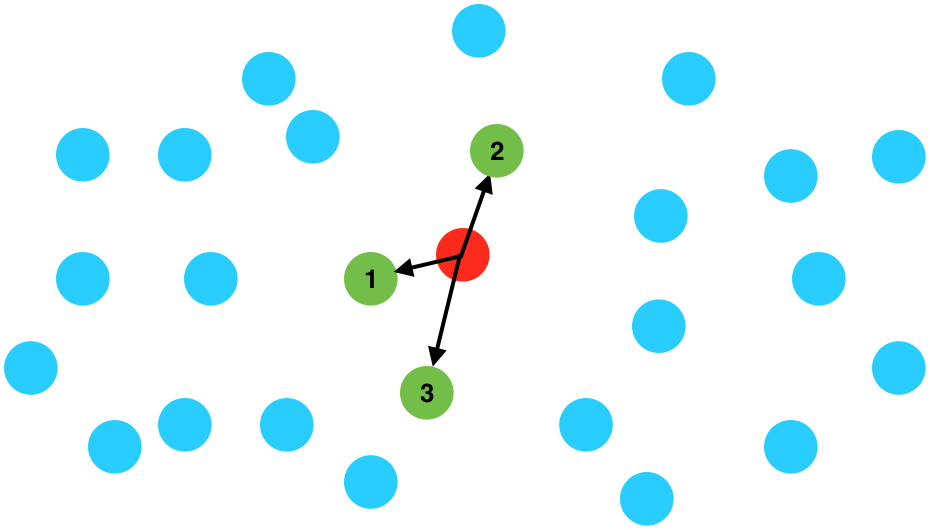
\includegraphics[width=350px]{assets/KnearestNeighbour}
	\caption{three nearest neighbors (points marked with green) of point (marked with red)}
\end{figure}

\subsection{Range and radius queries}
\paragraph{Problem Statement:} How do we retrieve all points inside a rectangle (range query) or circle (radius query) or any polygon.
\begin{figure}
	\centering
	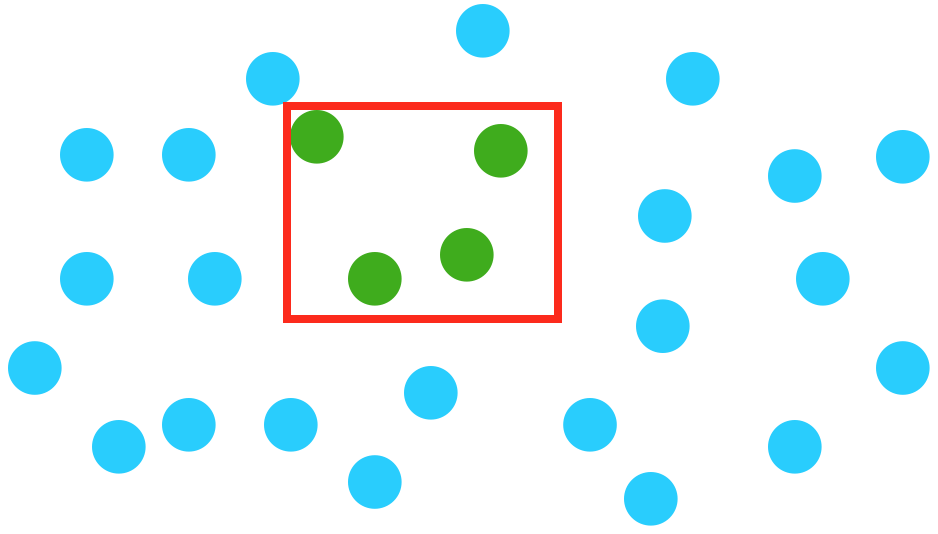
\includegraphics[width=350px]{assets/rangeAndRadius}
	\caption{three nearest neighbors (points marked with green) of point (marked with red)}
\end{figure}

\subsection{Solution - spatial trees}
\begin{itemize}
	\item Data changes are usually much less frequent than queries, so incurring an initial cost of processing data into an index is a fair price to pay for instant searches afterwards.
	\item Almost all spatial data structures share the same principle to enable efficient search: branch and bound. It means arranging data in a tree-like structure that allows discarding branches at once if they do not fit our search criteria.
\end{itemize}

\subsection{R-Tree}
\begin{figure}[htbp]
	\centering
	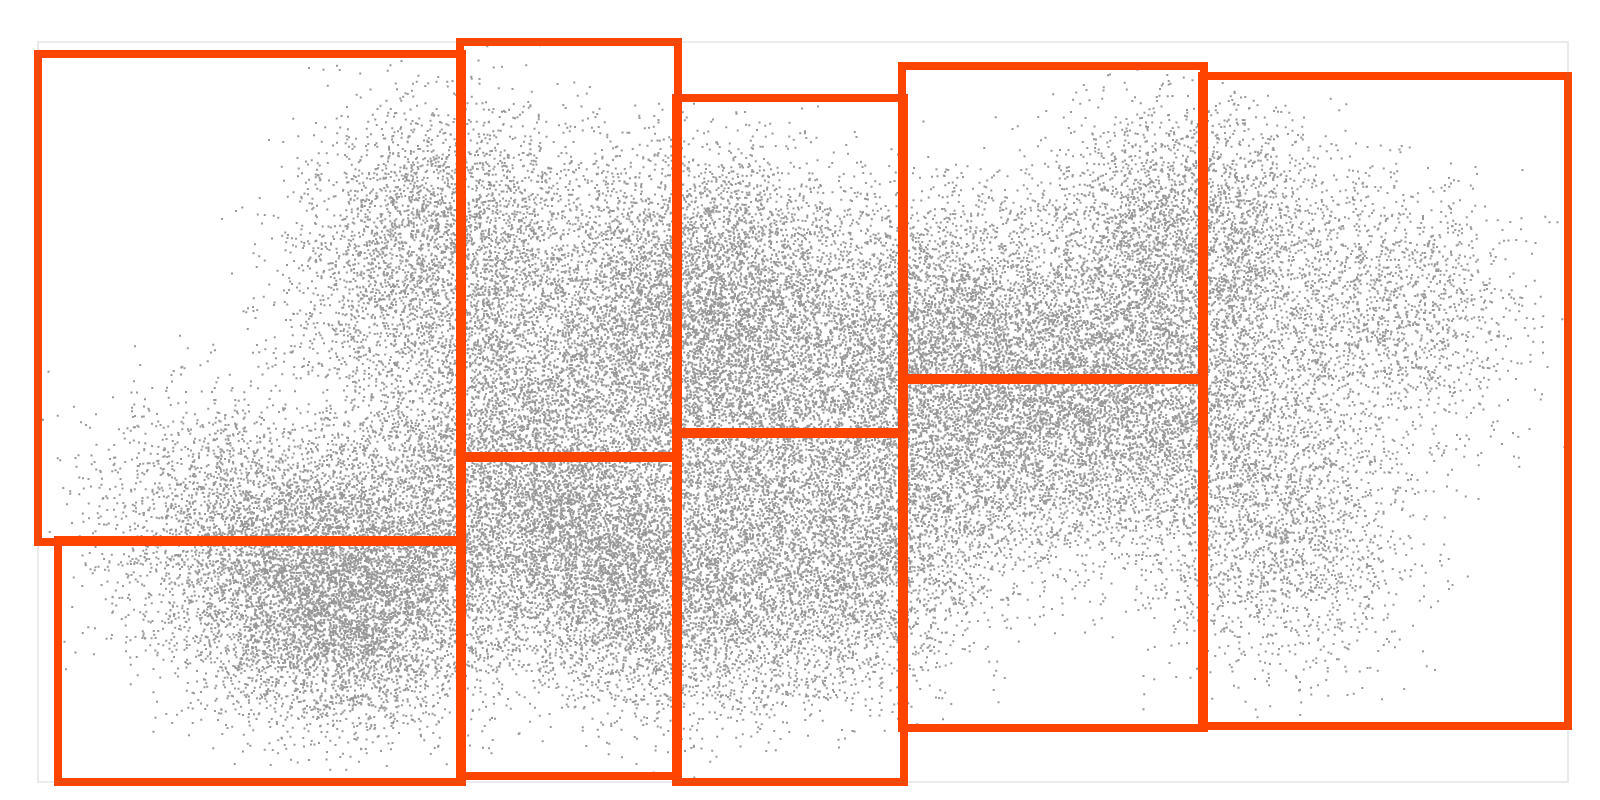
\includegraphics[width=350px]{assets/rtree1}
	\caption{sorted bunch of points in to rectangular boxes}
	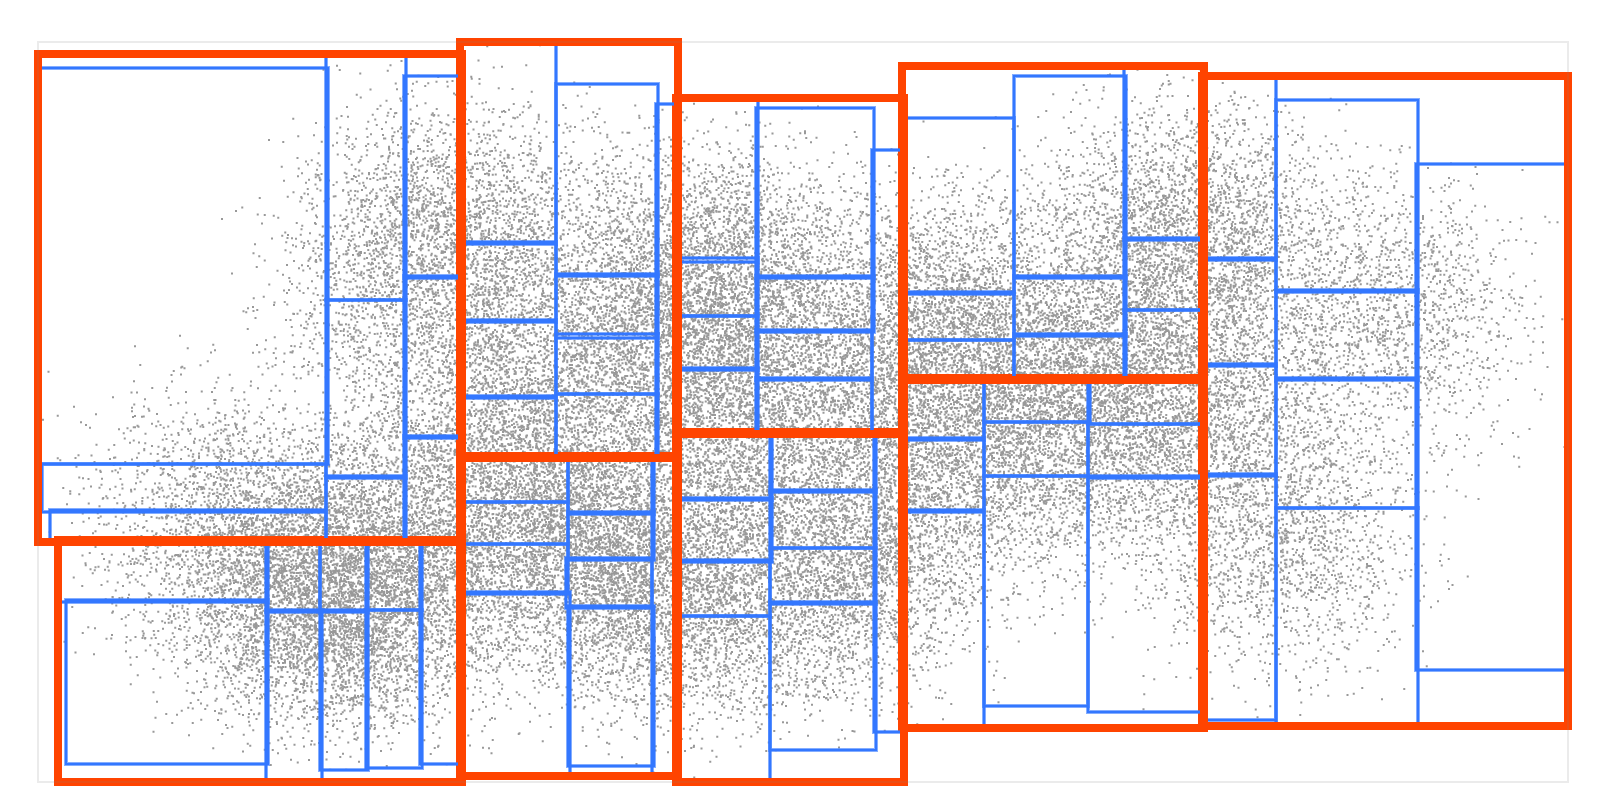
\includegraphics[width=350px]{assets/rtree2}
	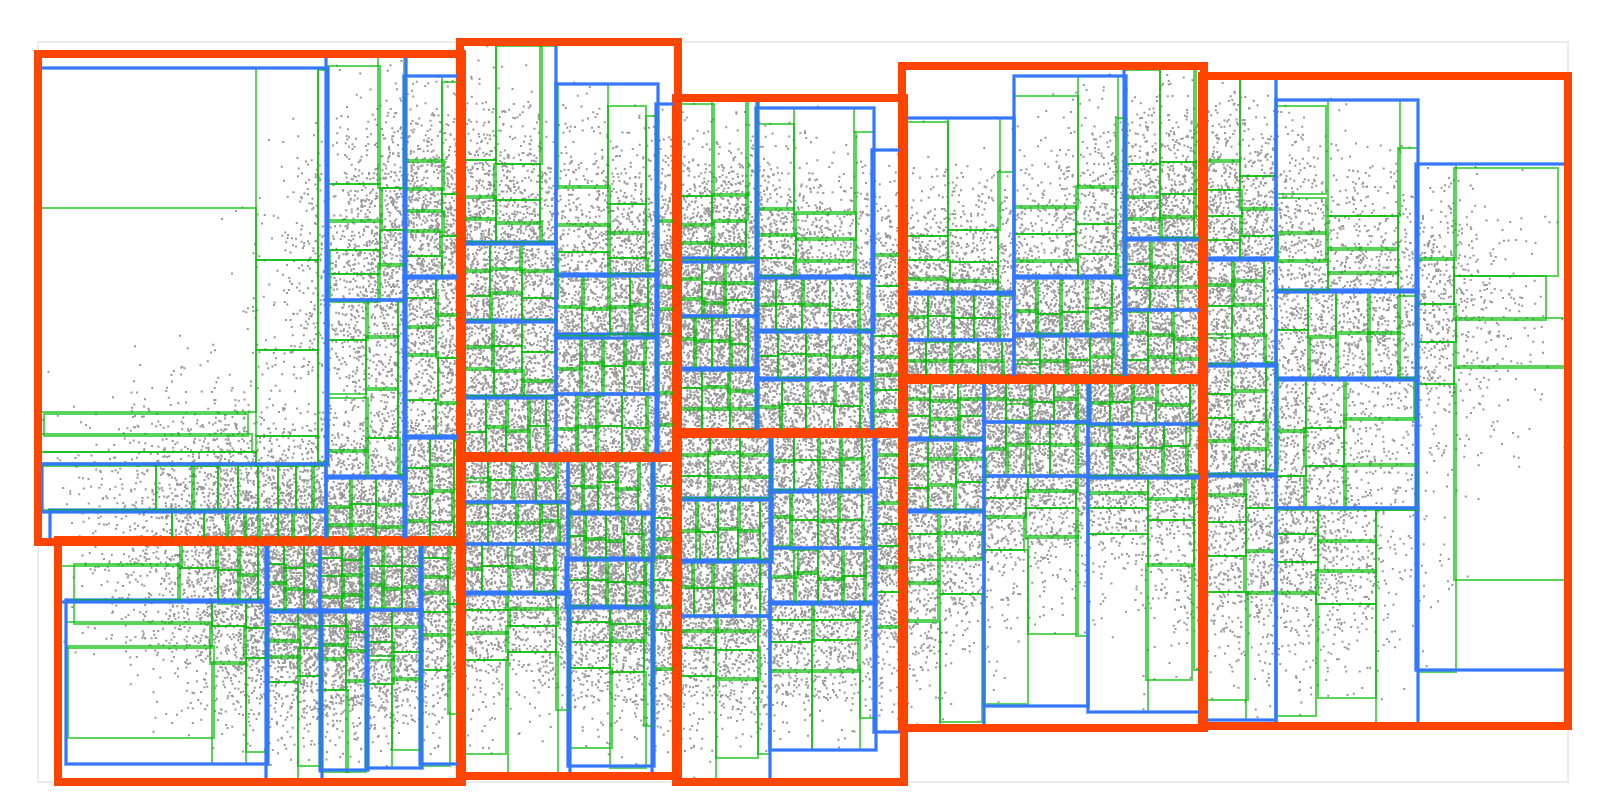
\includegraphics[width=350px]{assets/rtree3}
	\caption{further sorted bunch of points in to rectangular boxes from each rectangular box}
	\caption{R}
\end{figure}
\subsubsection{Trade off}
	\begin{itemize}
		\tick Quadtrees require fine-tuning by choosing appropriate tiling level in order to optimize performance. No specific tuning is required for R-Trees.
		\tick It’s used by all modern spatial databases and many game engines. 
		\tick R-trees are much faster than Quadtree for nearest neighbours queries.
		\tick R-trees are much faster than Quadtree for nearest neighbours queries.
		\fail Quadtree indexes are created faster than R-tree.
		\fail Quadtree can be implemented on top of existing B-tree. R-Tree -cannot
	\end{itemize}

\subsection{kd tree}
kd tree is similar to R-tree, but instead of sorting the points into several boxes at each tree level.
We sort them into two halves (around a median point) either left and right, or top and bottom, alternating between x and y split on each level
\begin{figure}[htbp]
	\centering
	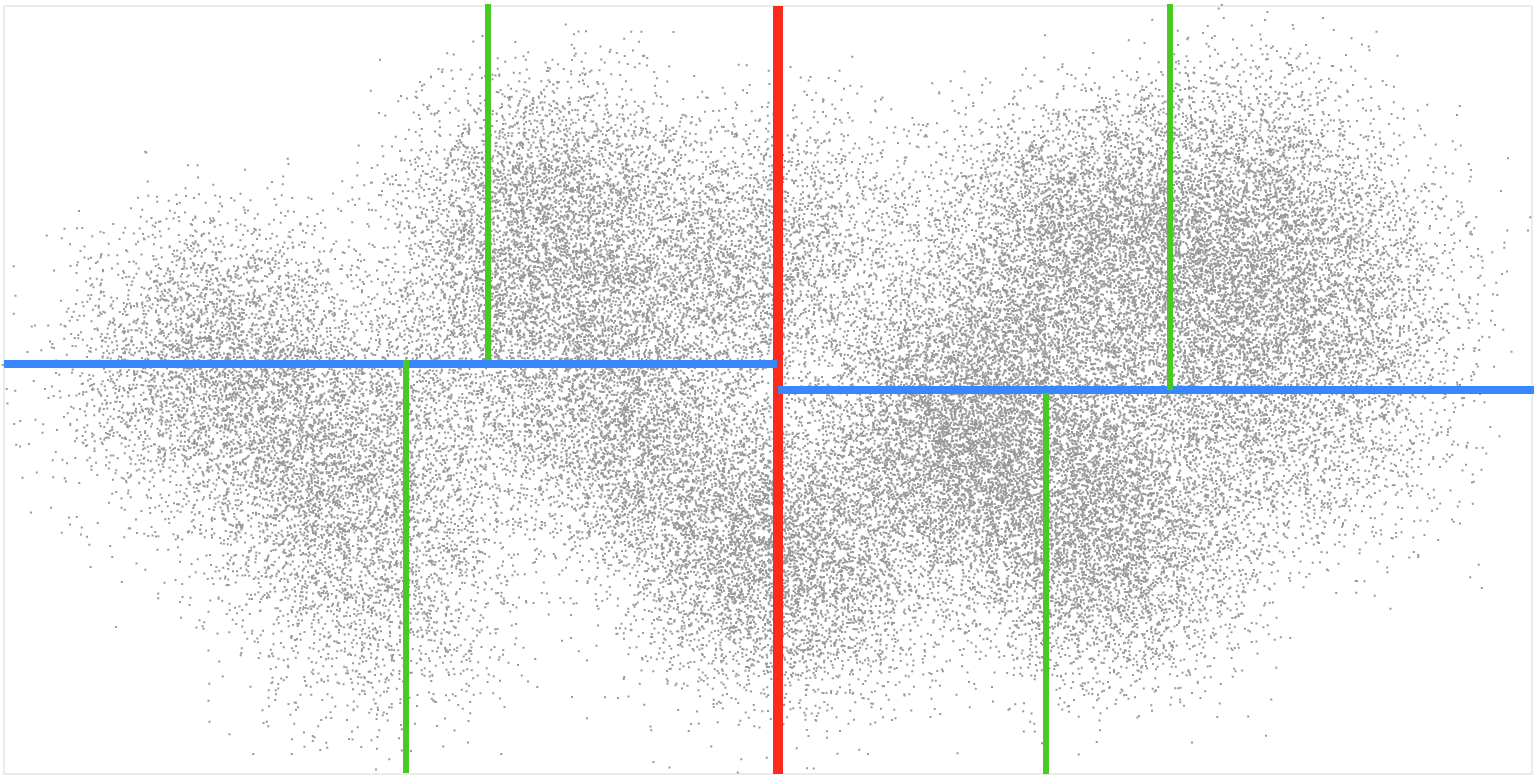
\includegraphics[width=350px]{assets/kd-tree}
	\caption{first three levels of kd tree}
	\caption{R}
\end{figure}
\begin{itemize}
	\fail Compared to R-tree, K-d tree can usually only contain points (not rectangles), and doesn’t handle adding and removing points. 
	\tick It’s much easier to implement, and it’s very fast.
\end{itemize}



%\setlength{\tabcolsep}{10pt} % Default value: 6pt
\renewcommand{\arraystretch}{2} % Default value: 1
\begin{table}[!ht]
	\caption{Feature Matrix for Multidimensional Indexed}
	\newcolumntype{P}{>{\centering\arraybackslash}m{2cm}}
	\newcolumntype{R}{>{\arraybackslash}m{2cm}}
	\begin{tabular}{ R | P P | P P P P }
	
	\hline
	Query & \multicolumn{2}{c| }{\textbf{Hash Based}}& \multicolumn{4}{c}{\textbf{Tree Based}}
	\\ \cline{2-7}
	Type & Grid & Partitioned Hash & MultiKey & kd-Tree & Quad Tree & R Tree 
	\\ \hline
	Exact Match & \good & \good & \good & \good & \good & Reasonable
	\\ \hline 
	Partial Match & \good & \good & works only for first key & \good & \good & \good
	\\ \hline 
	Range & \good & \bad & \bad & \good & \good & \good
	\\ \hline 
	Nearest Neighbour & \good & \bad & \bad & Reasonable & \good & Reasonable
	\\ \hline 
	Where am I & N/A & N/A & N/A & N/A & N/A & \good 
	\\ \hline 
	\hline
	Balanced Tree & N/A & N/A & \good & \bad & \bad & \good
	\\ \hline 
	\# of empty nodes or buckets & High (if large data file) & -- & -- & -- & High [Sol: keep only Not-NULL pointer only] & N/A
	\\ \hline 
	Splitting & Easy & Hard & N/A & N/A & N/A & N/A
	\\ \hline 
	Splitting Point & Distribute Data & N/A & N/A & any point that distribute data & centre point always & N/A
	\\ \hline 
	uniformly distributed data with a high change frequency &  &  &  &  & \good & \bad
	\\ \hline
	\end{tabular}
\end{table}


%----------------------------------------------------------------------------------------
%\end{multicols}
\end{document}
